Le robuROC 6 (\autoref{fig:01}) est un robot mobile développé par la société ROBOSOFT. Cette plate-forme robotisée a été conçue pour des applications de recherche et d’exploration en milieu extérieur. Elle est équipée de 6 roues motrices indépendantes, de même diamètre, montées par paires sur 3 podes articulés en tangage et en roulis (\autoref{fig:03}). La cinématique permet à la plate-forme de se conformer au relief parcouru et de franchir des obstacles du type trottoirs, escaliers… Le robuROC 6 a été conçu pour se déplacer en zones urbaines et peut aussi s’adapter à tous types de milieux.  Afin d’explorer la zone géographique à risques, les 3 podes peuvent être équipés, selon les besoins de l’utilisateur, de caméras d’observation haute définition à 360\degres, de systèmes infrarouges de visualisation nocturne, ainsi que de bras de robot articulés pour manipuler des éléments de la zone à explorer. Les diagrammes SADT A-0 (figure 1) et FAST (annexe 1) recensent les fonctions remplies par la plate-forme.

\begin{figure}
\centering
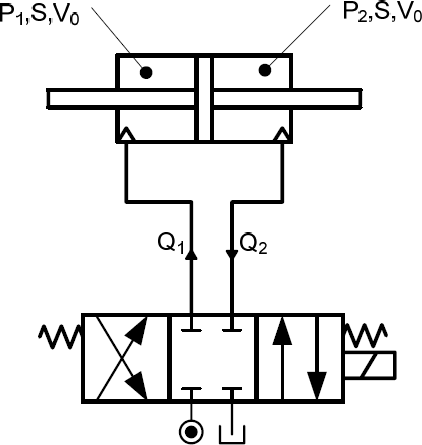
\includegraphics[width=.5\linewidth]{img_01}
\caption{RobuROC 6 \label{fig:01}}
\end{figure}

Les déplacements de la plate-forme sont coordonnés par l’intermédiaire de deux microcontrôleurs placés dans les podes avant et arrière. Ces microcontrôleurs communiquent entre eux et dialoguent avec l’extérieur suivant deux modes de conduite : 
\begin{itemize}
\item le mode joystick : l’utilisateur pilote manuellement la plate-forme par l’intermédiaire d’une télécommande;
\item le mode automatique : la plate-forme traite les informations du logiciel de supervision notamment le suivi d’un profil théorique.
\end{itemize}

Pour se repérer dans l’espace, la plate-forme est équipée de capteurs relatifs positionnés sur chacune des six roues, d’inclinomètres et d’un système de positionnement absolu par GPS. Des capteurs à ultrasons et des « bumpers » (détecteurs de collision) participent à la sécurité matérielle et à la détection des obstacles.
La motorisation principale est assurée par six moteurs électriques équipés de réducteurs épicycloïdaux permettant de transmettre l’énergie mécanique aux six roues. Le franchissement des obstacles est facilité par un système hydraulique permettant le soulèvement des podes avant et arrière. Ce système est constitué de quatre vérins disposés de part et d’autre du pode central (\autoref{fig:03}) et d’une centrale hydraulique alimentée par une pompe à engrenage (annexe 2). La plate-forme peut se déplacer, sous conditions, en mode 6 roues ou 4 roues pour certaines applications particulières (\autoref{fig:02}). L’énergie électrique nécessaire au fonctionnement est stockée dans des batteries occupant la plus grande partie du volume interne des trois podes. Une unité de gestion électrique optimise la consommation d’énergie. 

\begin{figure}
\centering
\begin{subfigure}{0.3\textwidth}
    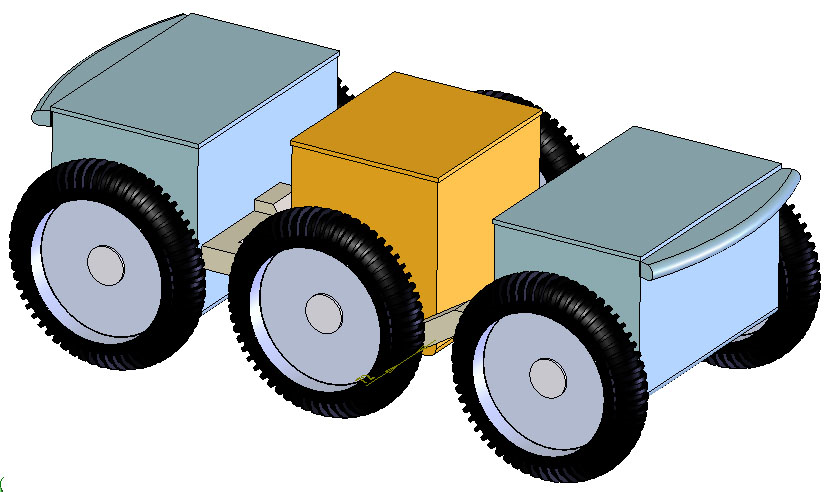
\includegraphics[width=\linewidth]{img_02_a}
    \caption{Mode 6 roues}
    \label{fig:02a}
\end{subfigure}
\begin{subfigure}{0.3\textwidth}
    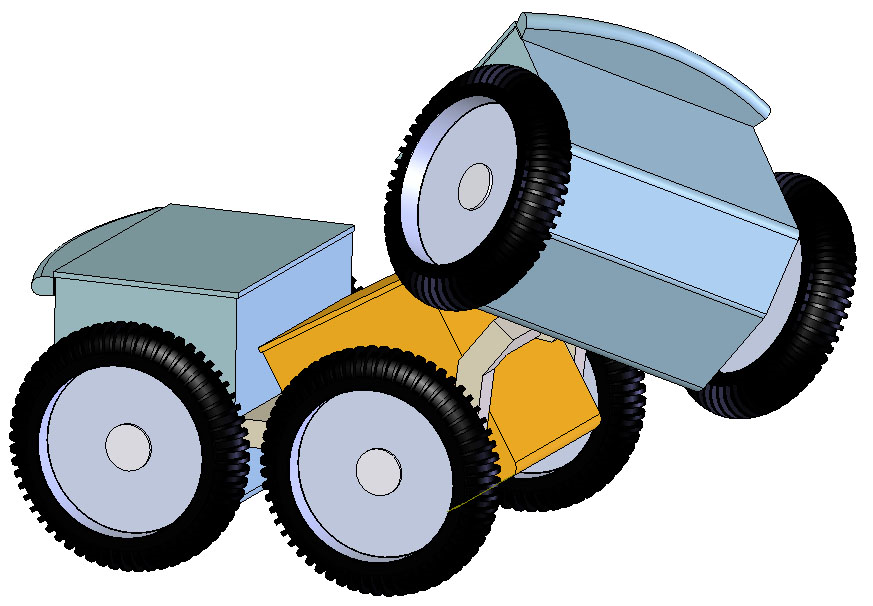
\includegraphics[width=\linewidth]{img_02_b}
    \caption{Mode 4 roues -- Déplacement}
    \label{fig:02a}
\end{subfigure}
\begin{subfigure}{0.3\textwidth}
    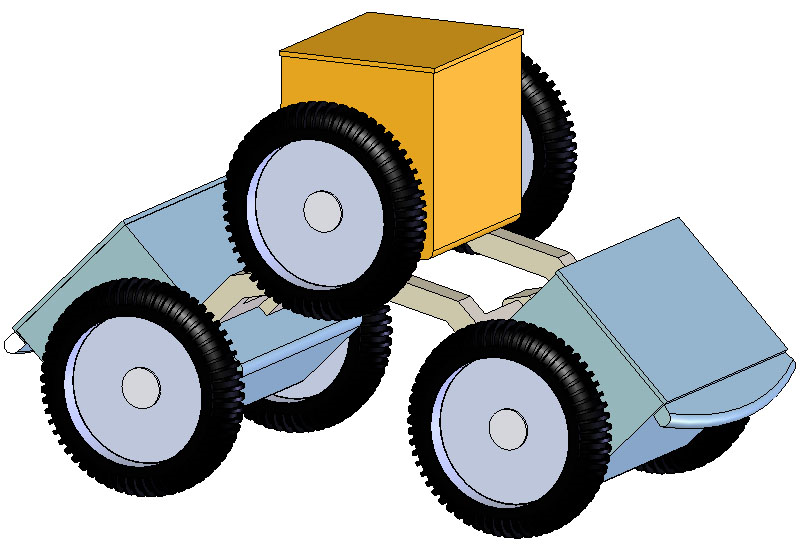
\includegraphics[width=\linewidth]{img_02_c}
    \caption{Mode 4 roues -- Observation}
    \label{fig:02a}
\end{subfigure}\caption{Mode de déplacement de la plate-forme \label{fig:02}}
\end{figure}


\begin{figure}
\centering
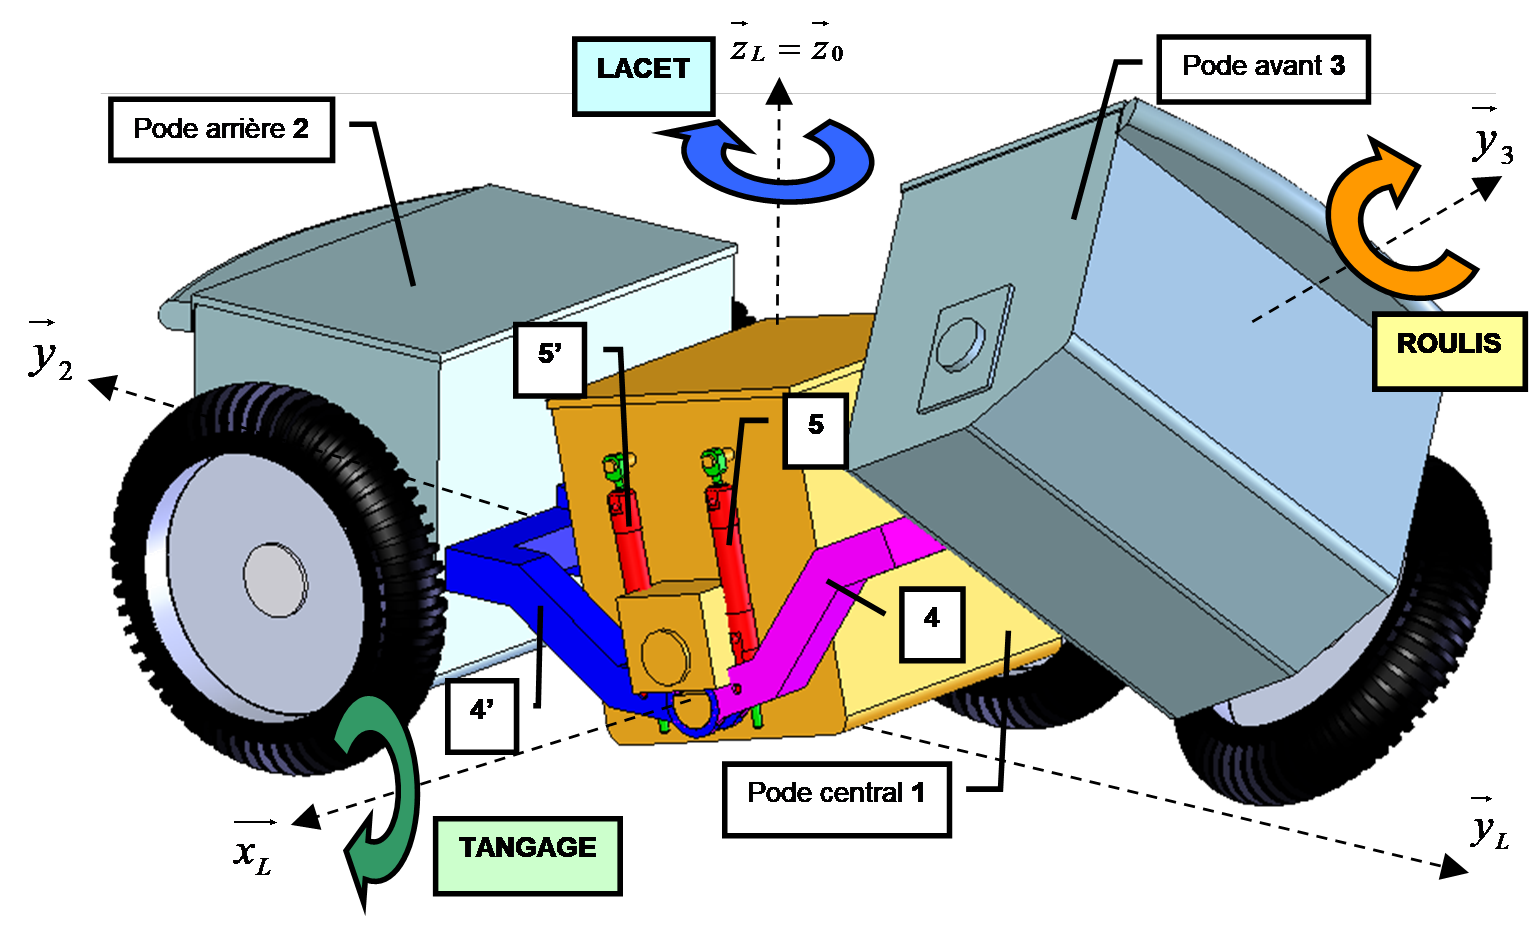
\includegraphics[width=.85\linewidth]{img_03}
\caption{Roue centrale et roue avant droite supprimées pour plus de visibilité \label{img:03}}
\end{figure}

Les trois podes sont articulés en tangage et en roulis (\autoref{fig:03}). Le mouvement de tangage est guidé par deux liaisons pivot (d’axe de direction  $\vect{x_L}$), respectivement entre le bras d’articulation avant \textbf{4} et le pode central \textbf{1} et entre le bras d’articulation arrière \textbf{4’} et le pode central \textbf{1}. Le système hydraulique de suspension permet l’amortissement (mode passif) et la motorisation de ce mouvement (mode actif). Les vérins \textbf{5} (côté droit) et \textbf{6} (côté gauche) sont en liaison avec le bras d’articulation avant \textbf{4} et le pode central \textbf{1}. Les vérins \textbf{5’} (côté droit) et \textbf{6’} (côté gauche) sont en liaison avec le bras d’articulation arrière \textbf{4’} et le pode central \textbf{1}. Le mouvement de roulis est assuré par deux liaisons pivot entre le pode avant \textbf{3} et le bras d’articulation avant \textbf{4} (liaison d’axe de direction $\vect{y_3}$) d’une part, et entre le pode arrière \textbf{2} et le bras d’articulation arrière \textbf{4’}  (liaison d’axe de direction $\vect{y_2}$) d’autre part. Ce mouvement n’est pas motorisé. 

\begin{table}
\centering
\begin{tabular}{|p{5cm}|p{5cm}|l|l|}
\hline
Fonctions & Critères & Niveaux & Flexibilité \\ 
\hline
\hline
FT3 : Assurer le déplacement	
 & Vitesse de déplacement de la plate-forme & $\SI{13,7}{km/h}$ & Valeur maximale \\ \cline{2-4}
 & Hauteur de franchissement d’un obstacle de type « trottoir » ($D_{\text{max}}$) & \SI{40}{cm} & Valeur minimale  \\ \cline{2-4}
 & Pente du relief à vide & 45\degres & Valeur maximale  \\ \cline{2-4}
 & Débattement angulaire en tangage du bras 4 par rapport au pode central 1 & de $-45\degres$ à $+30\degres$ & -----  \\ \cline{2-4}
 & Débattement angulaire en tangage du bras 4’ par rapport au pode central 1 & de $+45\degres$ à $-30\degres$ & ----- \\ \cline{2-4}
 & Débattement angulaire en roulis du pode avant 3 par rapport au bras 4 & de $-45\degres$ à $+45\degres$ & ----- \\ \cline{2-4}
 & Débattement angulaire en roulis du pode arrière 2 par rapport au bras 4’ & de $+45\degres$ à $-45\degres$ & ----- \\
 \hline
FT4 : Analyser la zone géographique à explorer
 & Charge utile répartie sur les trois podes & \SI{100}{kg} & Valeur maximale \\ \hline
 & Hauteur d’observation ($H_{\text{obs}}$) & \SI{85}{cm} & Valeur minimale \\ \hline
FT6 : Fournir l’énergie électrique & Autonomie d’utilisation $\SI{4}{h} $ & $\pm \SI{1}{h}$ &Selon les conditions \\ \hline
\end{tabular}
\caption{Extrait du cahier des charges fonctionnel (d’après le diagramme FAST en annexe 1)}
\end{table}

\section{Analyse fonctionnelle \label{sec:1}}
\question{\label{q_01} Compléter le diagramme FAST de la plate-forme d’exploration présenté en annexe 1 en indiquant les solutions techniques associées aux fonctions techniques référencées dans le tableau du document-réponse.}



\section{Fonction technique FT32 : Assurer le mouvement en tangage \label{sec:2}}

\begin{hypo}~\\
\begin{itemize}
\item Dans toute la partie II, le mouvement de roulis est fixé à une valeur nulle. Ainsi le bras d’articulation avant \textbf{4} et
le pode avant \textbf{3} sont solidaires et de la même manière, le bras d’articulation arrière \textbf{4’} et le pode arrière \textbf{2} sont
aussi solidaires. D’autre part, le mouvement de lacet n’est pas considéré.
\item Les éléments hydrauliques placés du côté gauche (vérins \textbf{6} et \textbf{6’}) agissent exactement de la même manière
que les éléments placés du côté droit (vérins \textbf{5} et \textbf{5’}). L’étude suivante du circuit hydraulique sera donc
réalisée uniquement du côté droit.
\end{itemize}
\end{hypo}

\subsection{Fonctionnement du circuit hydraulique}

Les fonctions à remplir par le circuit hydraulique (annexe 2) sont principalement de :
\begin{itemize}
\item synchroniser les mouvements de tangage des podes avant et arrière afin de se conformer au relief ;
\item amortir les mouvements de tangage ;
\item piloter les mouvements de tangage.
\end{itemize}

\subsubsection{Synchroniser et amortir les mouvements de tangage des trois podes}

Dans un premier temps, la centrale hydraulique n’est pas activée (annexe 2). Il s’agit donc d’étudier le comportement
de la plate-forme en mode passif (suivi du relief et amortissement des mouvements sans pilotage).
Les vérins utilisés, tous identiques, sont des vérins à double effet et tige traversante. Chaque vérin possède deux
chambres à volume variable remplies d’huile. Deux répartiteurs hydrauliques (un répartiteur placé du côté gauche et
l’autre du côté droit) assurent la circulation de l’huile entre les vérins avant et arrière en croisant l’alimentation des
chambres des vérins avant et arrière.

Un schéma cinématique du montage des vérins est fourni en annexe 3 et est complété par la représentation des
principales fonctionnalités du répartiteur hydraulique droit.


\question{\label{q_02}Sur le document-réponse (questions 2 et 3), indiquer en hachurant, les chambres des vérins qui sont en
communication ainsi que le flexible permettant de les relier. Vous adopterez un type de hachures par volume
d’huile en communication.}

À partir d’une position plane de la plate-forme (position du document-réponse questions 2 et 3), considérons que le
pode avant \textbf{3} commence un mouvement de CABRAGE (montée du pode avant \textbf{3} et du bras d’articulation \textbf{4} par rapport
au pode central \textbf{1}) suite à un obstacle. On note $\beta$ l’angle de tangage entre le bras d’articulation \textbf{4} et le pode central \textbf{1}
engendré par ce mouvement.

\question{\label{q_03}Sur le document-réponse (questions 2 et 3), indiquer par des flèches le sens de circulation de l’huile dans
les flexibles au cours de ce mouvement de CABRAGE. Indiquer quel est le mouvement engendré entre
l’ensemble \{pode arrière \textbf{2} + bras d’articulation \textbf{4’}\} et le pode central \textbf{1}, ainsi que son amplitude suite au
mouvement de CABRAGE du pode avant d’un angle $\beta$.}

\subsubsection{Piloter les mouvements de tangage}
Le système hydraulique est conçu de telle sorte que les angles de tangage entre le pode central \textbf{1} d’une part et les
podes avant / arrière d’autre part soient opposés à chaque instant. Ainsi, l’utilisateur n’a besoin de définir qu’un seul
angle de tangage $\beta$ défini entre le pode central \textbf{1} et le pode avant \textbf{3} par $\beta=\angl{y_1}{y_3}=\angl{z_1}{z_3}$ (annexe 5). L’angle
$\beta$
varie entre $- 45\degres$ et $+30\degres$. Les valeurs négatives correspondent à un mouvement de PLONGEE du pode avant, les
valeurs positives à un mouvement de CABRAGE.

Afin de piloter l’angle de tangage $\beta$ conformément aux consignes des microcontrôleurs, la centrale hydraulique est
activée. Un schéma de principe de cette centrale est fourni sur le document-réponse (question \ref{q_04}). La circulation
d’huile est générée par une pompe à engrenage entraînée par un moteur électrique. Les consignes électriques de
CABRAGE ou de PLONGEE agissent sur un distributeur 4/3 (4 orifices et 3 positions) afin de réaliser le mouvement
attendu au niveau des vérins (description du fonctionnement et de la normalisation d’un distributeur 4/3 disponible en
annexe 4).

\question{\label{q_04} Sur le document-réponse (question \ref{q_04}), relier les orifices de sortie du distributeur 4/3 aux flexibles
d’alimentation des vérins afin de respecter les ordres de PLONGEE et de CABRAGE.}

\subsection{Validation des performances du circuit hydraulique}

La position de PLONGEE maximale, permet au pode central \textbf{1} d’atteindre son point culminant par rapport au sol. Seuls
les podes avant \textbf{3} / arrière \textbf{2} sont alors en contact avec le sol horizontal. Cette position, appelée « Mode 4 roues
Observation » (\autoref{fig_02}), permet à l’utilisateur d’observer le milieu environnant à l’aide d’une caméra placée sur le plan
supérieur du pode central. La position de CABRAGE maximale, permet quant à elle de soulever le pode avant le plus
haut possible afin de franchir un obstacle (« Mode 4 roues Déplacement » (\autoref{fig_02})). Dans cette position, seuls le
pode arrière \textbf{2} et le pode central \textbf{2} sont en contact avec le sol.

\subsubsection{Etude du CABRAGE}

Sur le document-réponse (question \ref{q_05}), le pode central \textbf{1} est représenté en « Mode 4 roues Déplacement ». Les
podes \textbf{2} et \textbf{3} ont été représentés en pointillés dans leur position initiale pour un angle de tangage nul. Les points $C_{3i}$
et $C_{2i}$ définissent respectivement les positions initiales du centre de la roue avant et du centre de la roue arrière.

\question{\label{q_05}Représenter, sur le document-réponse (question \ref{q_05}), pour la position de CABRAGE maximal ($\beta_{\text{max}}=30\degres$) :\begin{itemize}
\item les positions du centre de la roue avant, appelé $C_{3C}$ et du centre de la roue arrière, appelé $C_{2C}$;
\item les cercles représentant les roues avant et arrière ainsi qu’une droite représentant le sol ;
\item la hauteur de franchissement maximal $D_{\text{max}}$ mesurée perpendiculairement au sol jusqu’au bas de la roue avant.
\end{itemize}
Mesurer $D_{\text{max}}$ et comparer cette valeur au cahier des charges.}

\subsubsection{Dimensionnement des vérins}
Le choix des vérins assurant le mouvement de tangage est délicat. En effet, l’encombrement très réduit oblige le
concepteur à positionner l’axe de fixation des vérins avec les bras \textbf{4} et \textbf{4’} très près de l’axe de rotation en
tangage $\axe{O_1}{x_L}$. L’objectif de cette partie est de déterminer la course des vérins en fonction de l’amplitude du
mouvement ainsi que la pression maximale $p_{\text{maxi}}$ dans le circuit hydraulique. Pour cette étude, nous considèrerons la
configuration d’essai suivante où le pode central \textbf{1} est fixe et placé parallèlement au sol. L’ensemble E=\{bras
d’articulation avant \textbf{4} + pode avant \textbf{3} + roues avant\} est soulevé par les vérins avant \textbf{5} et \textbf{6} placés de part et d’autre du
pode central \textbf{1}. Le modèle cinématique retenu est défini sur l’annexe 6.

Le mécanisme est constitué : 
\begin{itemize}
 \item du pode central fixe \textbf{1} : repère associé $\rep{1}=\repere{O_1}{x_1}{y_1}{z_1}$;
 \item de l'ensemble  E=\{bras d’articulation avant \textbf{4} + pode avant \textbf{3} + roues avant\} : repère associé $\rep{3}=\repere{O_1}{x_1}{y_3}{z_3}$ avec $\beta = \axe{y_1}{y_3} =\axe{z_1}{z_3}$;
 \item du vérin \textbf{4} constitué du corps \textbf{$5_1$} et de la tige \textbf{$5_2$} : repère associé $\rep{5}=\repere{A}{x_1}{y_5}{z_5}$ avec
  $\gamma = \axe{y_3}{y_5}= \axe{z_3}{z_5}$;
 \item du vérin \textbf{6} non représenté car ayant le même comportement que le vérin \textbf{5}.
\end{itemize}

Paramétrage : 
\begin{itemize}
 \item $\vect{O_1 A}=d_4\vect{y_3}$, $\vect{AB}=\lambda\vect{y_5}$, $\vect{O_1 B}=d_1\vect{y_1}+h_1\vect{z_1}$.
\end{itemize}

Valeurs numériques : 
\begin{itemize}
 \item $d_4 =\SI{70}{mm}$; $h_1 =\SI{292}{mm}$; $d_1 =\SI{76}{mm}$; $\beta \in \left[ -45\degres;+30\degres\right]$.
\end{itemize}

\question{Exprimer $\lambda$ en fonction de $d_4$, $h_1$, $d_1$ et $\beta$.}

\question{Calculer les valeurs numériques d’élongation minimale $\lambda_{\text{min}}$, maximale $\lambda_{\text{max}}$ ainsi que la course du vérin \textbf{5}.}

L’objectif suivant est d’évaluer les pressions maximales s’exerçant dans le circuit hydraulique dans la configuration
d’essai décrite précédemment à savoir :
\begin{itemize}
\item le pode central \textbf{1} est fixe et placé parallèlement au sol ;
\item les podes avant \textbf{3} et arrière \textbf{2} ne sont pas en contact avec le sol et un angle de tangage est alors imposé aux
podes avant et arrière par rapport au pode central.
\end{itemize}
Sur l’annexe 8, l’évolution du rapport entre les efforts exercés par les vérins avant \textbf{5} et \textbf{6} et le poids de l’ensemble E a
été tracée en fonction de l’angle de tangage $\beta$. La masse de l’ensemble E est $m_E = \SI{60}{kg}$.

\question{À partir du tracé de l’annexe 8 et du plan du vérin annexe 7, déterminer la valeur de la différence de
pression maximale $\Delta P_{\text{max}}$ entre les deux chambres des vérins avant \textbf{5} et \textbf{6}.}

La pression minimale dans le circuit hydraulique est supposée constante et égale à $p_0$ ( $p_0 = \SI{1}{bar}$). Des limiteurs de
pression tarés à \SI{150}{bars} sont placés en sortie du distributeur 4/3.

\question{Déterminer l’expression de la pression maximale $p_{\text{maxi}}$ dans le circuit hydraulique en fonction de $p_0$ et
$\Delta P_{\text{max}}$. Réaliser l’application numérique et comparer cette valeur à la pression de tarage des limiteurs.}

\section{Fonction technique FT31 : Assurer le mouvement de lacet}
Hypothèses :

\begin{itemize}
\item De la même manière que dans la partie \ref{sec:2}, dans toute la partie \ref{sec:3}, le mouvement de roulis n’est pas considéré.
Il est fixé à une valeur nulle.
\end{itemize}
Les 6 roues de la plate-forme (notée $PF$) sont motorisées permettant ainsi de se déplacer sur des reliefs très
accidentés. Cependant, la plate-forme ne comporte pas de systèmes spécifiques de direction. Le changement de
direction est imposé par une rotation différentielle des roues du pode central \textbf{1}. Les roues avant et arrière doivent alors
avoir des vitesses de rotation compatibles avec celles du pode central \textbf{1}. Lorsque le rayon de courbure de la trajectoire
suivie par la plate-forme devient inférieur à 4 mètres, le groupe hydraulique est actionné pour passer en « Mode 2
roues instable ». La plate-forme ne tenant pas en équilibre sur 2 roues, elle retombe dès le début du mouvement sur
les roues arrière ou les roues avant, passant donc en « Mode 4 roues Déplacement ». Cette intervention du groupe
hydraulique permet ainsi de soulager le contact entre les roues des podes avant / arrière et le sol. Pour cette étude,
nous considèrerons que la plate-forme retombe sur les roues arrière (annexe 9) et nous nous placerons dans le cas
d’un rayon de courbure nul. Le mouvement de lacet étudié est donc une rotation autour de l’axe $\axe{C_1}{z_0}$ d’angle $\varphi$,
appelé angle de lacet.

Ce mouvement est défini par le torseur cinématique suivant : 
$\torseurcin{V}{\text{PF}}{0} = \torseurl{\vecto{\text{PF}}{0}=\varphip \vect{z_0}}{\vect{0}}{C_1}$.

L’objectif de cette partie est de valider l’aptitude du système à respecter la
loi de vitesse de la \autoref{img:04}.
Le modèle cinématique retenu est représenté sur l’annexe 9.
Les roues centrales et les roues arrière sont en contact avec le sol. Dans ce
mode, seules les roues centrales $R_{1d}$ et $R_{1g}$ sont motrices. Elles roulent
sans glisser sur le sol en $I_{1d}$ et $I_{1g}$. Les roues du pode avant \textbf{3} et du pode
arrière \textbf{2} sont bloquées (\autoref{img:05}).

\begin{figure}[!h]
\centering
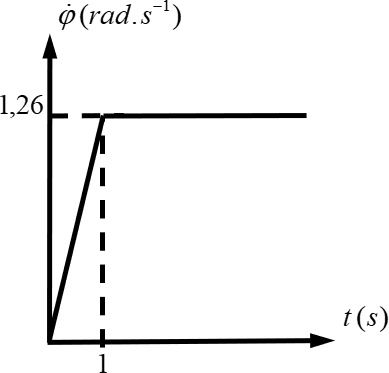
\includegraphics[width=.35\linewidth]{img_04}
\caption{Loi de commande de vitesse \label{img:04}}
\end{figure}

Paramétrage : (annexe 9)
\begin{itemize}
\item $\rep{0}=\repere{O_0}{x_0}{y_0}{z_0}$ lié au sol \textbf{0} et supposé << galiléen >>;
\item $\rep{L}=\repere{C_1}{x_L}{y_L}{z_L}$ lié à la plateforme PF tel que $\varphi=\angl{x_0}{x_L}=\angl{y_0}{y_L}$ appelé angle de lacet ;
\item $\rep{1}=\repere{C_1}{x_1}{y_1}{z_1}$ lié au pode central \textbf{1} tel que $\beta=\angl{y_L}{y_1}=\angl{z_L}{z_1}$; $\beta$ est l'angle de tangage, $\beta=2\degres$ (supposé constant pendant tout le mouvement du lacet);
\item $\rep{3}=\repere{C_3}{x_3}{y_3}{z_3}$ lié au pode avant \textbf{3} tel que $2\beta=\angl{y_L}{y_3}=\angl{z_L}{z_3}=4\degres$;
\item $\vect{C_1C_3}=b\vect{y_3}$ et $\vect{C_1C_2}=-b\vect{y_L}$ avec $b = \SI{553}{mm}$ ;
\item la \autoref{img:05} permet de définir le paramétrage de chacune des roues de la plate-forme en contact avec le sol avec
l’exemple de la roue centrale droite $R_{1d}$.
\end{itemize}

\begin{figure}[!h]
\centering
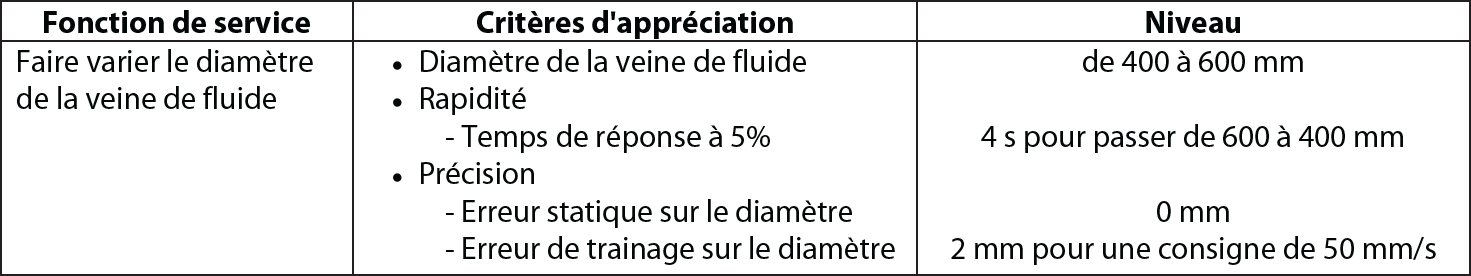
\includegraphics[width=.3\linewidth]{img_05}

\vspace{.5cm}

\begin{tabular}{lccccc}
\hline
&  & Centre & Point de & Vitesse de &  \\
&    Nom     &de         & contact  & rotation / au & Repère associé \\
&        & gravité & avec le sol & pode central & \\ \hline
Roue centrale droite & $R_{1d}$ & $C_{1d}$ & $I_{1d}$ & $\dot{\theta}_{1d}$ & $\rep{1d}=\repere{C_{1d}}{x_L}{y_{1d}}{z_{1d}}$ \\ \hline
Roue centrale gauche & $R_{1g}$ & $C_{1g}$ & $I_{1g}$ & $\dot{\theta}_{1g}$ & $\rep{1g}=\repere{C_{1g}}{x_L}{y_{1g}}{z_{1g}}$ \\ \hline
Roue arrière droite & $R_{2d}$ & $C_{2d}$ & $I_{2d}$ & & nulle \\ \hline
Roue arrière gauche & $R_{2g}$ & $C_{2g}$ & $I_{2g}$ & & nulle \\ \hline
\end{tabular}

\caption{Paramétrage des roues en contact avec le sol \label{img:05}}
\end{figure}





